%!TEX root = ../dissertation.tex

\chapter{Генерация детерминированных конечных автоматов при помощи уточнения абстракции по контрпримерам} 
\label{sec:cegar}

В настоящей главе описывается комбинированный метод генерации детерминированных конечных автоматов, на основе сведения к задаче выполнимости булевых формул и с использованием подхода уточнения абстракции по контрпримерам.

\section{Границы применимости (масштабируемость) предложенных методов в зависимости от размера расширенного префиксного дерева} % (fold)
\label{sec:cegar:motivation}

\inote{Методы, разработанные ранее супер! Но размер SAT формулы зависит от $N$ и $M$. Если $N$ (размер APTA) большое, то формула неудобоварима для солвера. Зачастую в примерах поведения содержится избыточная информация, которая ненужна для генерации соответствующего автомата. Вот, посмотрите, на пример. Куча примеров поведения, а автомат небольшой. Солвер не справляется, однако, если взять половину примеров поведения, то автомат строится за пару секунд. Но как понять какую половину нужно взять? Поможет CEGAR!}

Главной проблемой методов решения задачи построения минимального ДКА по примерам поведения при помощи сведения к SAT является размер получающейся формулы.
Ранее в~\cite{zakirzyanov2015LATA,zakirzyanov2017DataMode,zakirzyanov2019LATA} были предложены как более компактные способы кодирования поставленной задачи на языке SAT, так и различные подходы к сокращению пространства поиска. 
Тем не менее, подход, основанный на сведении к задаче выполнимости, все еще мало применим в случае, когда префиксное дерево
большое. Следует заметить, что префиксное дерево увеличивается в размере как при увеличении числа примеров поведения, так и при увеличении их длины.
В данном разделе описан новый подход к решению задачи построения минимального ДКА, позволяющий решить вышеуказанную проблему.
В случае, когда стоит задача построить некоторую модель, при этом имея доступ к проверяющей системе, часто применяется метод \emph{уточнения абстракции по контрпримерам} (\emph{Counterexample-Guided Abstraction Refinement}~--- CEGAR). 

\section{Метод генерации детерминированных конечных автоматов на основе сведения к задаче выполнимости и с использованием подхода уточнения абстракции по контрпримерам}
\label{sec:cegar:cegar-algo}

%далее копипаста
Суть данного метода можно описать следующим образом.
На начальном шаге генерируется некоторая, возможно случайная модель.
Затем на каждом следующем шаге данная модель проходит проверку некоторой проверяющей системы. Если проверка проходит успешно, то искомая модель найдена.
Иначе система возвращает один или несколько контрпримеров, которые затем используются для улучшения модели.
Процесс повторяется, пока не будет найдена модель, проходящая проверку системы.
Данный подход больше похож на метод активного построения модели, в то время как в данной работе рассматривается задача пассивного построения~--- все примеры поведения известны заранее и никакой дополнительной информации в ходе построения автомата быть получено не может.
Однако далее приводится описание того, как метод уточнения абстракции можно применить для построения ДКА.
%---------------

Как и классический алгоритм CEGAR, предлагаемый метод итеративно уточняет модель, которая в настоящей диссертации является детерминированным конечным автоматом.
Изначально расширенное префиксное дерево не содержит вершин, но будет достраиваться на каждом шаге.
На каждом шаге работы алгоритма предлагается с помощью сведения к SAT пытаться строить ДКА текущего размера по текущему префиксному дереву.
Если такой ДКА не существует, то как и раньше размер искомого автомата увеличивается на единицу и процесс поиска повторяется.
Если же такой автомат найден, он проверяется на соответствие всему множеству примеров поведения.
Если ДКА соответствует всем примерам поведения, то задача решена.
Иначе, среди тех примеров поведения, которым построенный автомат не соответствует, выбирается один или несколько контрпримеров, по которым достраивается префиксное дерево, строится новая булева формула и поиск продолжается.
Схема предложенного метода представлена на рисунке~\ref{img:cegar-algo}.

\begin{figure}[ht]
  \centering
  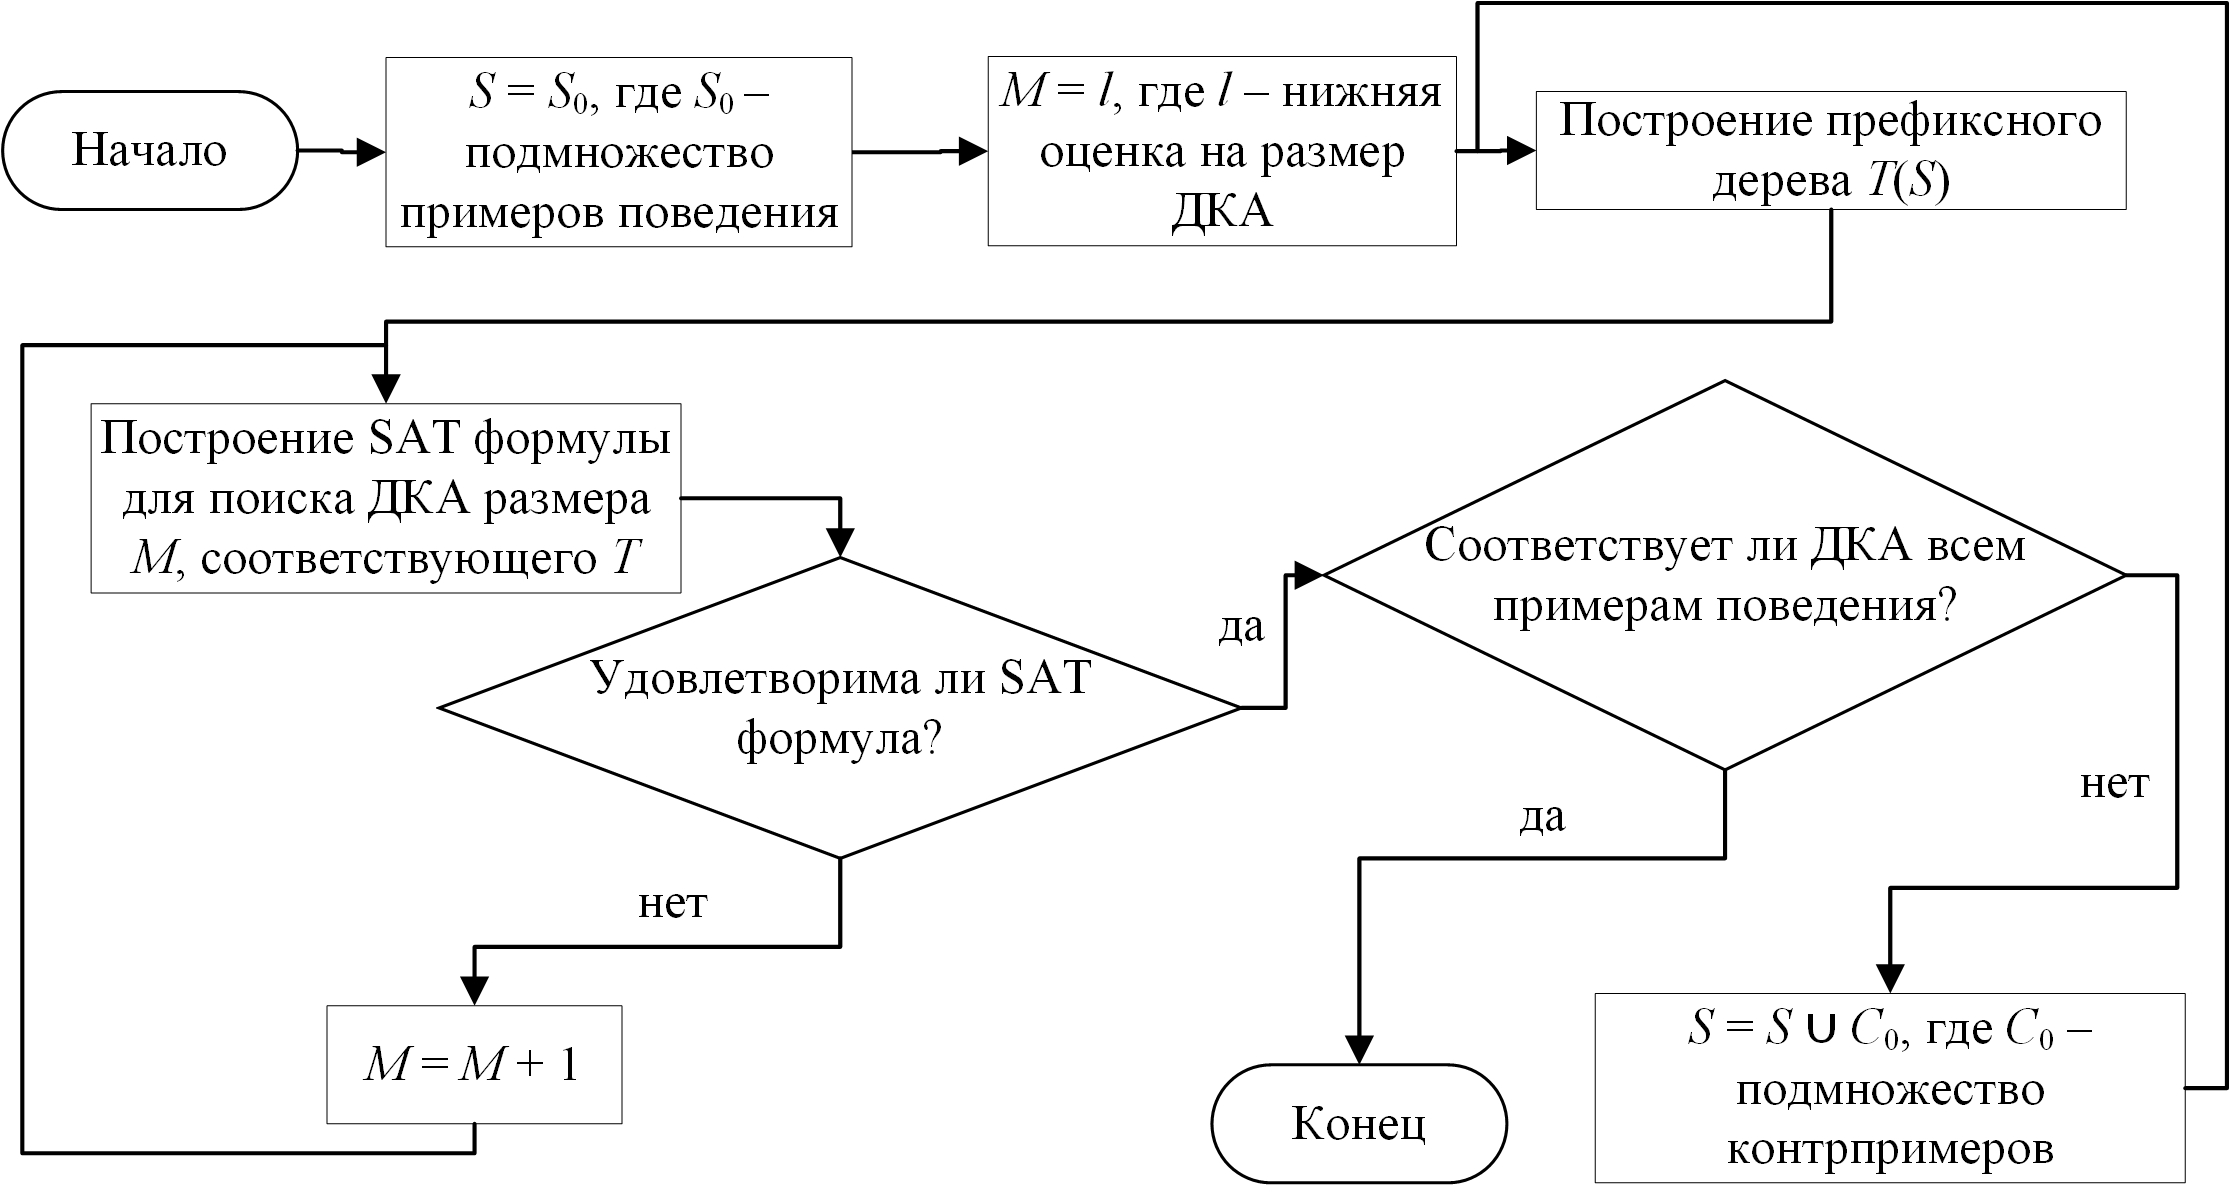
\includegraphics[scale=0.5]{img/ntv/cegar.jpg}
  \caption{Cхема точного метода генерации ДКА по избыточному набору примеров поведения на основе сведения к SAT и с использованием подхода CEGAR}
  \label{img:cegar-algo}
\end{figure}

Необходимо заметить, что перезапускать программное средство для решения SAT при каждом достраивании префиксного дерева крайне неэффективно, так как при добавлении новых дизъюнктов в формулу, пространство поиска решения SAT только сужается, а значит нет необходимости начинать поиск выполняющей подстановки заново.
Можно использовать инкрементальные программные средства, которые после нахождения некоторой выполняющей подстановки переходят в режим ожидания новых дизъюнктов и затем продолжают поиск решения уже для новой уточненной формулы с того места, где остановились в прошлый раз.


%----------------------------------------------------------------------------------------

\section{Реализация и экспериментальные исседования разработанного метода}
\label{sec:cegar:results}

В настоящем разделе приводятся описание реализации разработанных методов и экспериментальные исследования, проведенные с ними.

%----------------------------------------------------------------------------------------

\subsection{Реализация разработанного комбинированного метода генерации детерминированных конечных автоматов}
\label{sec:cegar:results:impl}

Предложенный в предыдущем разделе комбинированный метод построения ДКА минимального размера на основе сведения к SAT и с использованием подхода уточнения абстракции по контрпримерам был реализован на языке \emph{python} как модуль программного комплекса \texttt{DFA-Inductor-py}.

%----------------------------------------------------------------------------------------

\subsection{Экспериментальные исследования разработанного метода комбинированного метода генерации детерминированных конечных автоматов}
\label{sec:cegar:results:cegar}

%далее копипаста
Эксперименты проводились на персональном компьютере с процессором \emph{QuadCore Intel Core i7-8550U} @ 4 ГГц, 16 ГБ оперативной памяти и операционной системой \emph{ArchLinux 5.5.6}. Для проведения экспериментов было сгенерировано 100 тестовых экземпляров с помощью алгоритма, разработанного автором ранее и описанного в~\cite{zakirzyanov2017DataMode}.
Параметры для генерации автоматов были выбраны следующим образом:
\begin{itemize}
  \item размеры автоматов, которые нужно построить,~--- $M \in \left[15; 25\right]$;
  \item число примеров поведения $S = S_{+} \cup S_{-} \in \{50 \times N; 100 \times N; 200 \times N; 500 \times N\}$.
\end{itemize}
В экспериментах проводилось сравнение разработанного комбинированного метода с предложенным в~\cite{zakirzyanov2019LATA} методом, основанным только на сведении к SAT.
Результаты показали, что при относительно небольшом количестве примеров поведения ($S \in \{50 \times N; 100 \times N\}$) использование комбинированного подхода сокращает время построения вспомогательных структур данных (таких как граф совместимости) и время построения булевой формулы, но увеличивает время работы программного средства для решения SAT и, как следствие, суммарное время решения задачи.
Однако в случае, когда количество примеров поведения достаточно велико ($S \in \{200 \times N; 500 \times N\}$), использование предложенного подхода позволяет использовать меньше половины примеров поведения вместо всех, что сокращает как время построения структур данных и булевой формулы, так и время работы программного средства для решения SAT.
Выигрыш достигает $30 \%$ на экземплярах, которые оба метода смогли решить за 12 часов.
Значительная часть таких экземпляров не были в принципе решены методом, основанным только на сведении к SAT.
Таким образом, можно сделать вывод, что использование разработанного метода целесообразно, когда количество примеров поведения велико, и метод, основанный только на сведении к SAT, не применим ввиду слишком большой формулы.
%---------------

%----------------------------------------------------------------------------------------

\chresults{\ref{sec:cegar}}
